\documentclass[12pt,letterpaper]{article}
\usepackage{amsmath}
\usepackage{gensymb}
\usepackage{enumitem}
\usepackage{graphicx}
\usepackage[margin=1in]{geometry}
\setlength{\parindent}{0pt}
\title{Physics Club Practice Test 2}
\usepackage{titlesec}
\usepackage[export]{adjustbox}
\titlespacing{\paragraph}{0pt}{0pt}{1em}
% \setenumerate[2]{label={\alph*.}}
\usepackage{fancyhdr}
\fancypagestyle{firstpage}
{
	\renewcommand{\headrulewidth}{0pt}
	\rhead{Version 1.0}
	\cfoot{\thepage}
}
\thispagestyle{firstpage}
\begin{document}
\section*{Physics Club: $F=ma$ Practice Test 2}
Assume the acceleration due to gravity near the surface of the Earth $g = 10$ m/s$^2$.
\smallskip

Correct answers will be awarded one point; incorrect answers will result in a deduction of 1/4 point. There is no penalty for leaving an answer blank.
\smallskip

You may use a scientific calculator. Its memory must be cleared of data and programs.

\begin{enumerate}

\item
Consider a dripping faucet, where the faucet is 15 cm above the sink. The time between drops is such that when one drop hits the sink, one is in the air, and another is about to drop. At what height above the sink will the drop in the air be right as a drop hits the sink?
\begin{enumerate}
\item Between 2 and 4 cm
\item Between 4 and 6 cm
\item Between 6 and 8 cm
\item Between 8 and 10 cm
\item Between 10 and 12 cm
\end{enumerate}

\item
A cannonball is launched with initial velocity of magnitude $v_0$ over a horizontal surface. At what minimal angle $\theta_\text{min}$ above the horizontal should the cannonball be launched so that it rises to a height $H$ which is larger than one half of the horizontal distance $R$ that it will travel when it returns to the ground?
\begin{enumerate}
\item $\theta_\text{min} = 76\degree$
\item $\theta_\text{min} = 70\degree$
\item $\theta_\text{min} = 64\degree$
\item $\theta_\text{min} = 45\degree$
\item There is no such angle $\theta_\text{min}$, as $R>2H$ for all range problems.
\end{enumerate}

\item
An equilateral triangle is sitting on an inclined plane. Friction is too high for it to slide under any circumstance, but if the plane is sloped enough it can ``topple'' down the hill. What angle incline is necessary for it to start toppling?
\begin{enumerate}
\item 30 degrees
\item 45 degrees
\item 60 degrees
\item It will topple at any angle more than zero
\item It can never topple if it cannot slide
\end{enumerate}

\item
A particle at rest explodes into three particles of equal mass in the absence of external forces. Two particles emerge with velocities of the same magnitude $v$ but form an angle of $60\degree$. What is the speed of the third particle?
\begin{enumerate}
\item $v$
\item $\sqrt{3}v$
\item $2v$
\item $2\sqrt{3}v$
\item The third particle can have a range of different speeds.
\end{enumerate}

\item
A 12 kg block moving east at 3 m/s collides head on with a 6 kg block that is moving west at 2 m/s. The two blocks move together after the collision. What is the loss in kinetic energy in this collision?
\begin{enumerate}
\item 36 J
\item 50 J
\item 60 J
\item 72 J
\item 96 J
\end{enumerate}
\end{enumerate}

\textbf{The following information is used for questions X and Y.}\\
Two cannons are arranged vertically, with the lower cannon pointing upward (toward the upper cannon) and the upper cannon pointing downward (toward the lower cannon), 200 m above the lower cannon. Simultaneously, they both fire. The muzzle velocity of the lower cannon is 35 m/s and the muzzle velocity of the upper cannon is 55 m/s.

\begin{enumerate}[resume]
\item
How long after the cannons fire do the projectiles collide?
\begin{enumerate}
\item 2.2 s
\item 2.5 s
\item 3.6 s
\item 6.7 s
\item 8.0 s
\end{enumerate}

\item
How far beneath the top cannon do the projectiles collide?
\begin{enumerate}
\item 31 m
\item 67 m
\item 110 m
\item 150 m
\item 170 m
\end{enumerate}

\item
A block of mass $m = 4.0$ kg is moving on a horizontal surface toward a massless spring with spring constant $k = 80.0$ N/m. The coefficient of kinetic friction between the block and the surface is $\mu_k = 0.50$. The block has speed of 2.0 m/s when it first comes into contact with the spring. How far will the spring be compressed?
\begin{enumerate}
\item 0.19 m
\item 0.24 m
\item 0.32 m
\item 0.45 m
\item 0.61 m
\end{enumerate}

\item
A uniform spherical planet has radius $R$ and the acceleration due to gravity at its surface is $g$. What is the escape velocity of a particle from the planet's surface?
\begin{enumerate}
\item $\frac{1}{2}\sqrt{gR}$
\item $\sqrt{gR}$
\item $\sqrt{2gR}$
\item $2\sqrt{gR}$
\item The escape velocity cannot be expressed in terms of $g$ and $R$ alone.
\end{enumerate}

\item
Four objects are placed at rest at the top of an inclined plane and allowed to roll without slipping to the bottom in absence of rolling resistance and air resistance.\\
Object A is a solid brass ball of diameter $d$.\\
Object B is a solid brass ball of diameter $2d$.\\
Object C is a hollow brass sphere of diameter $d$.\\
Object D is a solid aluminum ball of diameter $d$. (Aluminum is less dense than brass.)\\
The balls are placed so that their centers of mass all travel the same distance. In each case, the time of motion $T$ is measured. Which of the following statements if correct?
\begin{enumerate}
\item $T_\text{B} > T_\text{C} > T_\text{A} = T_\text{D}$
\item $T_\text{A} = T_\text{B} > T_\text{C} = T_\text{D}$
\item $T_\text{B} > T_\text{A} = T_\text{C} = T_\text{D}$
\item $T_\text{A} = T_\text{B} = T_\text{C} = T_\text{D}$
\item $T_\text{C} > T_\text{A} = T_\text{B} = T_\text{D}$
\end{enumerate}

\item
As shown, Lily is using the rope through a fixed pulley to move a box with constant speed $v$. The kinetic friction coefficient between the box and the ground is $\mu <1$; assume that the fixed pulley is massless and there is no friction between the rope and the fixed pulley. Then, while the box is moving, which of the following statements is correct?
\begin{enumerate}
\item The magnitude of the force on the rope is constant.
\item The magnitude of friction between the ground and the box is increasing.
\item The magnitude of the normal force of the ground on the box is decreasing.
\item The pressure of the box on the ground is increasing.
\item The pressure of the box on the ground is constant.
\end{enumerate}

\item
A rigid hoop can rotate about the center. Two massless strings are attached to the hoop, one at A, the other at B. These strings are tied together at the center of the hoop at O, and a weight G is suspended from that point. The strings have a fixed length, regardless of the tension, and the weight G is only supported by the strings. Originally OA is horizontal and OB forms an angle $\theta_0 < 90\degree$ with the horizontal as shown in the diagram.\\

Now, the outer hoop will start to slowly rotate $90\degree$ clockwise until OA will become vertical, while keeping the angle between the strings constant and keeping the object static. Which of the following statements about the tensions $T_1$ and $T_2$ in the two strings is correct?
\begin{enumerate}
\item $T_1$ always decreases.
\item $T_1$ always increases.
\item $T_2$ always decreases.
\item $T_2$ always increases.
\item $T_2$ first increases then decreases.
\end{enumerate}

\item
Shown below is a graph of the $x$ component of force versus position for a 2.0 kg cart constrained to move in one dimension on the $x$ axis. At $x=0$ the cart has a velocity of $-3.0$ m/s (in the negative direction). Which of the following is closest to the maximum speed of the cart?
\begin{enumerate}
\item 5.1 m/s
\item 4.2 m/s
\item 4.0 m/s
\item 3.0 m/s
\item 2.5 m/s
\end{enumerate}

\item
A uniform cylinder of radius $a$ originally has a weight of 80 N. After an off-axis cylinder hole at $2a/5$ was drilled through it, it weighs 54 N. The axes of the two cylinders are parallel and their centers are at the same height.\\

A force $T$ is applied to the top of the cylinder horizontally. In order to keep the cylinder at rest, the magnitude of the force $T$ is closest to
\begin{enumerate}
\item 3 N
\item 5 N
\item 10 N
\item 25 N
\item 35 N
\end{enumerate}

\item
A car of mass $m$ has an engine that provides a constant power output $P$. Assuming no frictional loss of energy, what is the maximum constant speed $v_\text{max}$ that this car can drive up a long incline that makes an angle $\theta$ with the horizontal?
\begin{enumerate}
\item $\displaystyle v_\text{max} = \frac{1}{\sin\theta}\sqrt\frac{2P}{mg}$
\item $\displaystyle v_\text{max} = \frac{P^2\sin\theta}{mg}$
\item $\displaystyle v_\text{max} = \frac{P}{mg\sin\theta}$
\item There is no maximum constant speed.
\item The maximum constant speed depends on the length of the incline.
\end{enumerate}

\item
Inside a cart that is accelerating horizontally at acceleration $a$, there is a block of mass $M$ connected to two light springs of force constants $k_1$ and $k_2$. The block can move without friction horizontally. Find the vibration frequency of the block.
\begin{enumerate}
\item $\displaystyle \frac{1}{2\pi}\sqrt{\frac{k_1+k_2}{M}+a}$
\item $\displaystyle \frac{1}{2\pi}\sqrt{\frac{k_1+k_2}{M}}$
\item $\displaystyle \frac{1}{2\pi}\sqrt{\frac{k_1k_2}{(k_1+k_2)M}}$
\item $\displaystyle \frac{1}{2\pi}\sqrt{\frac{k_1k_2}{(k_1+k_2)M}+a}$
\item $\displaystyle \frac{1}{2\pi}\sqrt{\frac{|k_1-k_2}{M}}$
\end{enumerate}

\item
Shown below is a log-log plot for the data collected of amplitude and period of oscillation for a certain non-linear oscillator.\\

According to the data, the relationship between the period $T$ and the amplitude $A$ is best given by
\begin{enumerate}
\item $T = 100A^3$
\item $T = 1000A^2$
\item $T = 1000A$
\item $T = 2A + 3$
\item The period is independent of the amplitude for oscillating systems.
\end{enumerate}

\item
A mass hangs from the ceiling of a box by an ideal spring. With the box held fixed, the mass is given an initial velocity and oscillates with purely vertical motion. When the mass reaches the lowest point of its motion, the box is released and allowed to fall. To an observer inside the box, which of the following statements is true? Ignore air resistance.
\begin{enumerate}
\item The amplitude of the oscillation decreases.
\item The period of the oscillation increases.
\item The maximum speed reached by the mass increases.
\item The height, measured from the bottom, at which the mass reaches its maximum speed decreases.
\item The maximum height reached by the mass decreases.
\end{enumerate}

\item
A 1500 watt motor is used to pump water a vertical height of 2.0 meters out of a flooded basement through a cylindrical pipe. The water is ejected through the end of the pipe at a speed of 5.0 m/s. Ignoring friction and assuming that all of the energy of the motor goes to the water, which of the following is closest to the radius of the pipe? The density of water is 1000 kg/m$^3$.
\begin{enumerate}
\item 1/3 cm
\item 1 cm
\item 5 cm
\item 10 cm
\item 30 cm
\end{enumerate}

\item
A container of water is sitting on a scale. Originally, the scale reads $M_1 = 45$ kg. A block of wood is suspended from a second scale; originally the scale reads $M_2 = 12$ kg. The density of wood is 0.60 g/cm$^3$; the density of the water is 1.00 g/cm$^3$. The block of wood is lowered into the water until half of the block is beneath the surface. What is the resulting reading on the scales?
\begin{enumerate}
\item $M_1 = 55$ kg and $M_2 = 6$ kg
\item $M_1 = 55$ kg and $M_2 = 2$ kg
\item $M_1 = 45$ kg and $M_2 = 2$ kg
\item $M_1 = 45$ kg and $M_2 = 6$ kg
\item $M_1 = 45$ kg and $M_2 = 10$ kg
\end{enumerate}

\item
A spring system is set up as follows: a platform with a weight of 10 N is on top of two identical springs, each with spring constant 75 N/m. On top of the platform is a third spring with spring constant 75 N/m. If a ball with a weight of 5.0 N is then fastened to the top of the third spring and then slowly lowered, by how much does the height of the spring system change?
\begin{enumerate}
\item 0.033 m
\item 0.067 m
\item 0.100 m
\item 0.133 m
\item 0.600 m
\end{enumerate}

\item
The softest audible sound has an intensity of $I_0 = 10^{-12}$ W/m$^2$. In terms of fundamental units of kilograms, meters, and seconds, this is equivalent to
\begin{enumerate}
\item $I_0 = 10^{-12}$ kg/s
\item $I_0 = 10^{-12}$ kg$^2\,\cdot\,$m/s
\item $I_0 = 10^{-12}$ kg$^2\,\cdot\,$m/s$^2$
\item $I_0 = 10^{-12}$ kg$\,\cdot\,$m$^{-1}\,\cdot\,$s$^{-3}$
\item $I_0 = 10^{-12}$ kg/s$^3$
\end{enumerate}

\item
Which of the following sets of equipment cannot be used to measure the local value of the acceleration due to gravity ($g$)?
\begin{enumerate}
\item A spring scale (which reads in force units) and a known mass
\item A rod of known length, an unknown mass, and a stopwatch
\item A launcher which launches projectiles at a known speed, a projectile of known mass, and meter stick.
\item An inclined plane of known inclination, several carts of different known masses, and a stopwatch
\item A motor with a known output power, a known mass, a piece of string of unknown length, and a stopwatch
\end{enumerate}

\item
Three point masses $m$ are attached together by identical springs. When placed at rest on a horizontal surface the masses form a triangle with side length $l$. When the assembly is rotated about its center at angular velocity $\omega$, the masses form a triangle with side ength $2l$. What is the spring constant $k$ of the sprngs?
\begin{enumerate}
\item $2m\omega^2$
\item $\displaystyle \frac{2}{\sqrt{3}}m\omega^2$
\item $\displaystyle \frac{2}{3}m\omega^2$
\item $\displaystyle \frac{1}{\sqrt{3}}m\omega^2$
\item $\displaystyle \frac{1}{3}m\omega^2$
\end{enumerate}

\item
Consider the two orbits around the Sun shown below. Orbit P is circular with radius R, orbit Q is elliptical such that the farthest point b is between $2R$ and $3R$, and the nearest point a is between $R/3$ and $R/2$. Consider the magnitudes of the velocity of the circular orbit $v_\text{c}$, the velocity of the comet in the elliptical orbit at the farther point $v_\text{b}$, and the velocity of the comet in the elliptical orbit at the nearest point $v_\text{a}$. Which of the following rankings is correct?
\begin{enumerate}
\item $v_\text{b} > v_\text{c} > 2v_\text{a}$
\item $2v_\text{c} > v_\text{b} > v_\text{a}$
\item $10v_\text{b} > v_\text{a} > v_\text{c}$
\item $v_\text{c} > v_\text{a} > 4v_\text{b}$
\item $2v_\text{a} > \sqrt{2}v_\text{b} > v_\text{c}$
\end{enumerate}
%---------------

% \item
% Starting from rest at time $t = 0$, a car moves in a straight line with an acceleration given by the accompanying graph. What is the speed of the car at $t = 2$ s?

% \begin{tabular}{l r}

% \begin{minipage}{0.575\textwidth}
% \begin{enumerate}
% \item 1.0 m/s
% \item 2.0 m/s
% \item 8.0 m/s
% \item 10.5 m/s
% \item 12.5 m/s
% \end{enumerate}
% \end{minipage} &
% \begin{minipage}{0.4\textwidth}
% 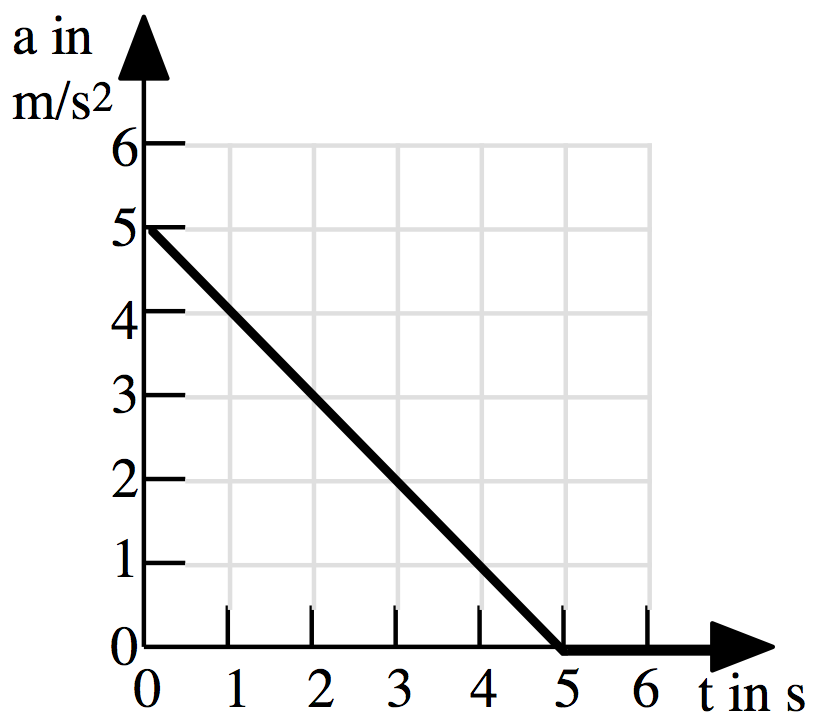
\includegraphics[width=0.65\textwidth,center]{agraph.png}
% \end{minipage}
% \end{tabular}
% \end{enumerate}

% \textbf{The following information is used for questions 2 and 3.}\\
% A flare is dropped from a plane flying over level ground at a velocity of 70 m/s in the horizontal direction. At the instant the flare is released, the plane begins to accelerate horizontally at 1.75 m/s$^2$. The flare takes 4.5 s to reach the ground.

% \begin{enumerate}[resume]
% \item
% Relative to a spot directly under the flare at release, the flare lands
% \begin{enumerate}
% \item directly on the spot.
% \item 333 m in front of the spot.
% \item 274 m in front of the spot.
% \item 280 m in front of the spot.
% \item 315 m in front of the spot.
% \end{enumerate}

% \vfill
% \newpage

% \item
% Which solid vector in the accompanying figures best represents the acceleration of the pendulum mass at the intermediate point in its swing indicated?

% 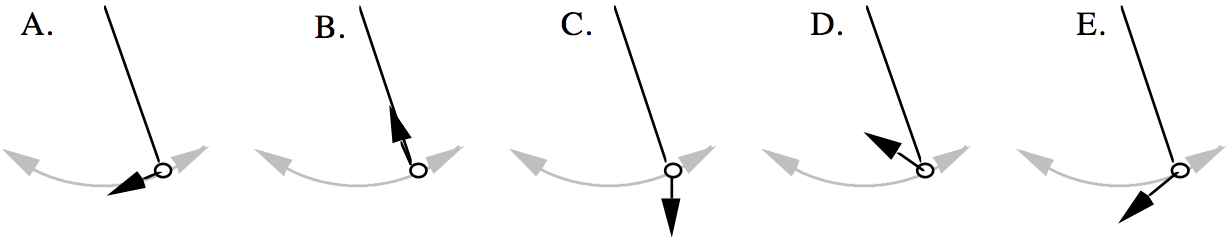
\includegraphics[width=0.9\textwidth,center]{swing.png}

\end{enumerate}

\end{document}
